%! suppress = TooLargeSection
\documentclass[conf]{new-aiaa}
%\documentclass[journal]{new-aiaa} for journal papers

% \usepackage{lgrind}
% \usepackage{cmap}
% \usepackage[T1]{fontenc}

\usepackage{microtype}
\usepackage{amsmath}
\let\Bbbk\relax
\usepackage{amssymb}
\usepackage{gensymb}
\usepackage{graphicx}
\usepackage{pgf}
\usepackage{float}
% \usepackage{optidef}
\usepackage{ifdraft}
\usepackage[hyphens]{url}
\usepackage{hyperref}
\usepackage{enumitem}

\renewcommand{\labelitemii}{$\circ$}

\usepackage{eqexpl}
\eqexplSetIntro{where:} % set parenthesis in the left of the first item
\eqexplSetDelim{=} % set delimiter to "="

\usepackage{ar}

\usepackage{multicol}

\usepackage{siunitx}
\sisetup{}

\usepackage{longtable}
\usepackage{tabularx}
\usepackage{booktabs}
\usepackage{multirow}
\usepackage{tablefootnote}
\usepackage{tabularray}
\UseTblrLibrary{booktabs}
\UseTblrLibrary{counter}

% \usepackage{mdframed}
% \newmdenv[
%     topline=false,
%     bottomline=false,
%     skipabove=\topsep,
%     skipbelow=\topsep,
%     innerleftmargin=30pt,
%     innerrightmargin=30pt,
%     backgroundcolor=black!5
% ]{example}

% \usepackage{fontspec}
% \usepackage{mathspec}
%\setmathsfont(Digits,Latin,Greek)[Numbers={Proportional}]{EB Garamond}
% \setmathrm{EB Garamond}

\widowpenalty=300
\clubpenalty=300
\interfootnotelinepenalty=10000
\tolerance=9999
\emergencystretch=10pt
\hyphenpenalty=1000
\exhyphenpenalty=100

% \defaultfontfeatures{Mapping=tex-text}
% \newfontfamily{\smallcaps}[RawFeature={+c2sc,+scmp}]{EB Garamond}
% \setromanfont[Numbers={Proportional}, Ligatures={Common}]{EB Garamond}
% \setsansfont[Scale=MatchLowercase, BoldFont={Lato Bold}]{Lato Regular}
% \setmonofont[Scale=MatchLowercase]{Source Code Pro}



\usepackage{tikz}
\usetikzlibrary{positioning}
\usetikzlibrary{shapes.geometric}
\usetikzlibrary{shapes.arrows}
\usetikzlibrary{decorations.pathmorphing, decorations.pathreplacing, calc}
\usetikzlibrary{arrows.meta, positioning}

\usepackage{tikz-cd}
\tikzcdset{
    math mode=false
}

% \usepackage{minted}
% \usemintedstyle{pastie}
% %\usemintedstyle{jupyter_python}
% %\usemintedstyle{rainbow_dash}
% %\usemintedstyle{colorful}
% \setminted{
%     frame=lines,
%     framesep=2mm,
% %    numbers=left,
%     fontsize=\footnotesize,
% %    fontsize=\scriptsize,
%     autogobble=true,
%     baselinestretch=1.15,
%     breaklines,
%     linenos,
%     highlightcolor=cyan!15,
% }
% \setmintedinline{
%     breaklines
% }

% \PassOptionsToPackage{table,xcdraw}{xcolor}
\usepackage{xcolor}

% \definecolor{c1}{HTML}{64ACBE}
% \definecolor{c2}{HTML}{EE442F}
% \definecolor{c3}{HTML}{601A4A}

\definecolor{myorange}{RGB}{255, 165, 0}
\definecolor{mydarkseagreen}{RGB}{143, 188, 143}
\definecolor{mydodgerblue}{RGB}{30, 144, 255}

\colorlet{b}{red!13!white}
\colorlet{m}{yellow!20!white}
\colorlet{g}{green!18!white}


% \renewcommand{\theFancyVerbLine}{\sffamily
%     \textcolor[rgb]{0.8,0.8,0.8}{\scriptsize\oldstylenums{\arabic{FancyVerbLine}}}
% }


\usepackage{titlesec}
%\newcommand{\sectionbreak}{\clearpage}

\usepackage{caption}
\captionsetup[table]{skip=6pt}

\usepackage[numbers,sort&compress]{natbib}

\usepackage{adjustbox}

\usepackage[titletoc,title]{appendix}

% \usepackage{geometry}
% \geometry{
%     letterpaper,
%     left=1.0in,
%     right=1.0in,
%     top=1.0in,
%     bottom=1.0in
% }

% \usepackage{setspace}
% \setstretch{2}

\usepackage[inkscapearea=page]{svg}

\usepackage{subcaption}

\usepackage{afterpage}
\usepackage[section]{placeins}

\usepackage{nth}

%\usepackage{titling}
% \usepackage[palatino,nogrey]{quotchap}
% \definecolor{chaptergrey}{HTML}{64ACBE}


\usepackage{xstring}

% \makeatletter
%     \patchcmd{\@makechapterhead}{\thechapter}{%
%      \IfSubStr{ABCDEFGHIJKLMNOPQRSTUVWXYZ}{\thechapter}{\appname\,\thechapter}{\chapname\,\thechapter}
%     }
% \makeatother

% \newcommand{\appname}{{\fontfamily{phv}\fontsize{22pt}{26pt}\selectfont\raisebox{1em}{\textcolor{gray}{Appendix}}}} % set the appendix name <<<<<<<<<<<
% \newcommand{\chapname}{{\fontfamily{phv}\fontsize{22pt}{26pt}\selectfont\raisebox{1em}{\textcolor{gray}{\chaptername}}}} % set the chapter name <<<<<<<<<<<

\usepackage{authblk}

\usepackage{todonotes}
\setuptodonotes{inline,backgroundcolor=yellow!20,prepend,caption={TODO}}

\newcommand{\Rey}{\rm Re}
\newcommand{\M}{\rm M}
\newcommand{\Cp}{C_p}
\newcommand{\Cpo}{C_{p_0}}
\newcommand{\Cpm}{C_{p_{\rm min}}}
\newcommand{\Cpom}{C_{p_{0,\rm min}}}
\newcommand{\Cpcr}{C_{p_{\rm crit}}}
\newcommand{\Mcr}{M_{\rm crit}}
\newcommand{\Mdd}{M_{\rm dd}}
\newcommand{\Mi}{M_\infty}
\newcommand{\Ncr}{N_{\rm crit}}

\title{NeuralFoil: An Airfoil Aerodynamics Analysis Tool Using Physics-Informed Machine Learning}

\author{Peter Sharpe\footnote{PhD Candidate, AIAA Student Member} and R. John Hansman\footnote{T. Wilson Professor in Aeronautics, AIAA Fellow}}
\affil{Massachusetts Institute of Technology, Cambridge, MA}

\begin{document}

    \maketitle

    \begin{abstract}

        This work introduces \emph{NeuralFoil}, an open-source tool for rapid aerodynamics analysis of airfoils, similar to XFoil. NeuralFoil uses a physics-informed machine learning approach, with physics constraints structurally embedded into the model architecture and training performed on tens of millions of XFoil runs. Compared to XFoil, this allows nearly-identical aerodynamic accuracy, runtime speeds up to 1,000x faster on large batch analyses, and most importantly, compatibility with gradient-based design optimization methods (e.g., infinitely-smooth solutions, no non-convergence issues, and straightforward compatibility with automatic differentiation tools). NeuralFoil yields airfoil aerodynamics results including viscous and compressible effects for nearly any practical airfoil, including control deflections, across a full $360\degree$ range of angles of attack, across Reynolds numbers from $10^2$ to $10^9$, and for Mach numbers from zero to low transonic conditions. This work discusses the architecture, training, and performance of NeuralFoil on a variety of test cases, including an airfoil design optimization case for the MIT Daedalus human-powered aircraft. In this case study, NeuralFoil optimization is able to produce airfoils remarkably similar in performance and shape to expert-designed airfoils in seconds; this provides a good starting point for further expert refinement. NeuralFoil is implemented as a lightweight Python package with minimal dependencies, allowing easy installation across a variety of platforms.

    \end{abstract}

    \section{Nomenclature}

    {\renewcommand\arraystretch{1.0}
    \noindent\begin{longtable*}{@{}l @{\quad=\quad} p{5in}@{}}
                 $\beta$ & Prandtl-Glauert compressibility correction factor, defined as $\sqrt{1 - \Mi^2}$ \\
                 BL & boundary layer \\
                 CFD & computational fluid dynamics \\
                 $C_D$ & drag coefficient \\
                 $C_L$ & lift coefficient \\
                 $C_M$ & moment coefficient \\
                 $\Cp$ & local pressure coefficient (in the real compressible flow) \\
                 $\Cpo$ & local pressure coefficient in the equivalent incompressible flow \\
                 $\Cpm$ & minimum local pressure coefficient (in the real compressible flow) \\
                 $\Cpom$ & minimum local pressure coefficient in the equivalent incompressible flow \\
                 $c$ & airfoil chord \\
                 $c_\mathcal{D}$ & dissipation coefficient \\
                 $c_f$ & skin friction coefficient \\
                 $c_{\rm lower}$ & Kulfan (CST) shape parameters associated with the airfoil's lower surface \\
                 $c_{\rm upper}$ & Kulfan (CST) shape parameters associated with the airfoil's upper surface \\
                 $\gamma$ & ratio of specific heats of the working fluid; 1.4 for air near standard conditions \\
                 $H$ & BL shape parameter, defined as $\delta^*/\theta$ \\
                 $H^*$ & BL kinetic energy shape parameter, defined as $\theta^*/\theta$ \\
                 LE & leading edge \\
                 $M$ & local Mach number \\
                 $\Mi$ & freestream Mach number \\
                 $\Mcr$ & critical Mach number, defined as the lowest freestream Mach number where any point in the flow is supersonic \\
                 $M_{\rm dd}$ & drag-divergent Mach number, defined as the freestream Mach number above which drag begins to rise rapidly \\
                 RANS & Reynolds-averaged Navier-Stokes \\
                 TE & trailing edge \\
                 $u_\infty$ & freestream velocity magnitude \\
                 $u_{\rm max}$ & maximum velocity magnitude at any point in the flow field \\
                 $x_{\rm tr}$ & laminar-turbulent transition location, relative to the leading edge; appropriate suffixes denote top- and bottom-surface measures \\
                 $x / c$ & nondimensional distance along the airfoil chord ($\text{LE} \rightarrow 0$, $\text{TE} \rightarrow 1$) \\
                 $y / c$ & nondimensional distance normal to the airfoil chord (LE and TE at 0, barring any control surface deflections) \\
    \end{longtable*}}


    \section{Introduction}

    In conceptual aircraft design, the problem of shaping a typical wing can be decomposed into two parts: planform design and airfoil design. The latter, which is the focus of this work, is a multidisciplinary design problem that requires consideration of a variety of aerodynamic, structural, and manufacturing objectives and constraints. A non-exhaustive list of major considerations could include:
    \begin{itemize}
        \item Profile drag across the expected operating range of the airfoil (spanning lift coefficients, Reynolds numbers, and Mach numbers), including adequate off-design performance \cite{drela_pros_1998};
        \item Pitching moment coefficients, which can drive tail sizing (modifying trim drag) and affect divergence speed;
        \item Hinge moments and control effectiveness of any control surfaces, which drive actuator design and weight;
        \item Stall behavior, which can affect handling qualities and safety;
        \item Thickness at various points, in order to accommodate fuel volume and required structural members to resist failure (e.g., by bending, buckling, divergence, flutter, or control reversal);\cite{sharpe_tailerons_2023}
        \item Sensitivity to boundary layer performance, which places constraints on surface finish, cleanliness, and manufacturing tolerances \cite{eleshaky1993airfoil, selig_highlift_1997, liebeck1973class};
        \item Peak suction pressures, which affect the critical Mach number in transonic applications or cavitation in hydrodynamic applications;
        \item Shock stability and buffet considerations in transonic applications;
        \item Manufacturability, which might include flat-bottom airfoil sections, strictly-convex airfoil shapes (e.g., to accommodate shrink-coverings, which are common in ultra-lightweight applications \cite{drela_lowreynoldsnumber_1988}), or restrictions on trailing-edge angle.
    \end{itemize}

    These airfoil requirements often differ considerably at different points along the span of the wing, which often leads to a family of airfoils being used in the design of a given wing. To fulfill such design requirements, a designer will typically either find an existing airfoil or design a new airfoil. Given the specificity of the requirements illustrated in the list above, the latter is often necessary.

    Three approaches are commonly used to computationally design new airfoils: inverse design methods, direct manual methods, and optimization methods. In the inverse design approach, popularized by Drela's XFoil code \cite{drela_xfoil_1989} and Eppler's Profil code \cite{profil, tao_bs_thesis}, conformal mapping methods are used to reconstruct a new airfoil shape from a desired pressure distribution. This has the benefit of allowing the engineer to directly operate on the most relevant aerodynamic quantities, but it can struggle to produce airfoils that satisfy non-aerodynamic constraints (e.g., manufacturability) due to the lack of direct control here. Conformal mapping methods are also only applicable to potential-flow-governed regions, so the specified pressure distribution is often the inviscid, rather than viscous (true) pressure distribution\footnote{This can be alleviated by using nonlinear optimization to target the viscous pressure distribution, albeit with reduced numerical robustness.}.

    In the direct manual method (or ``geometric design'' method, using parlance from XFoil), an engineer formulates an airfoil shape directly and modifies this iteratively by hand. Aerodynamic analysis is performed by any code that will perform the forward problem (geometry $\rightarrow$ aerodynamics), such as XFoil, MSES \cite{mses}, or any RANS-based CFD code \cite{adler_cfd_2022}. This allows for easier satisfaction of non-aerodynamic constraints, but it is difficult to directly target aerodynamic quantities. Significant user expertise is also required to identify the most relevant geometric parameters and to make effective changes to the airfoil shape.

    In the optimization approach, a parameterized airfoil shape is optimized to minimize a cost function and satisfy specified constraints. At first glance, this appears to be an automation of the direct manual method. However, Drela and others note the surprising difficulty of posing the correct optimization problem \cite{drela_pros_1998, kroo_multidisciplinary_1997}, so this approach requires just as much (if not more) human expertise than the direct manual method. As stated by Drela \cite{drela_pros_1998}, optimization-based airfoil design ``is still an iterative cut-and-try undertaking. But compared to [direct] techniques, the cutting-and-trying is not on the geometry, but rather on the precise formulation of the optimization problem.'' To support this, Drela gives compelling case studies of how airfoil design optimization can go awry in the absence of user review and care. Some codes, like the LINDOP \cite{mses} optimization routine coupled with XFoil, alleviate this somewhat by using a hybrid of the direct and optimization approaches: update directions are computed by an optimizer, but the actual changes are reviewed and implemented by a human between iterations. Despite the potential challenges of this optimization-based airfoil design approach, it offers compelling benefits: resulting airfoil performance is competitive with expert-designed airfoils \cite{drela_pros_1998}, and optimization can provide a systematic and robust approach that solves challenging design problems from poor initial guesses \cite{he2019robust}.

    In all of these methods, some form of a computational tool for airfoil aerodynamics analysis is required. For subsonic airfoils, the gold standard of such tools is XFoil \cite{drela_xfoil_1989}. XFoil is more accurate than RANS-CFD-based tools \cite{morgado2016xfoil}, yet it has a computational cost that is roughly 1,000x lower -- a testament to the power of its modeling approach, which couples integral boundary layer and potential flow methods. A complete description of this modeling approach is available in Drela's \textit{Aerodynamics of Viscous Fluids} \cite{drela_aerodynamics_2019}, and in recent state-of-the-art work by Zhang \cite{zhang_threedimensional_2022, zhang_nonparametric_2017}. However, XFoil has several attributes that make it less-than-ideal for directly driving numerical optimization studies:

    \begin{itemize}
        \item XFoil is not guaranteed to produce a solution. When an ``ambitious'' calculations are attempted, XFoil often fails to provide a converged solution; the unconverged result often has wildly-diverging values and is effectively unusable. In some cases, calculations can lead to infinite loops or process crashes due to unhandled exceptions. While this is acceptable in certain applications (e.g., manual direct analysis), it is generally unacceptable for use in numerical optimization. Instead, optimization strongly benefits from a robust analysis tool that always produces a result, even if that result has slightly degraded accuracy. This allows the analysis to steer the optimizer back towards the design space of reasonable airfoils \cite{he2019robust}. A particularly useful case is when the model is deliberately made to be slightly pessimistic (e.g., overestimate drag) in regions of the design space with high uncertainty, adding further optimization pressure towards reasonable designs.
        \begin{itemize}
            \item More generally, design optimization is not the only application that strongly benefits from an aerodynamics analysis tool that always produces an answer. Other examples where a non-answer, infinite loop, or crashed process are unacceptable include real-time control (e.g., as an aerodynamic model for a model-predictive controller onboard an aircraft) and flight simulation.
        \end{itemize}
        \item XFoil solutions are not necessarily unique, and slightly different solutions can be obtained for the same analysis problem (airfoil shape, angle of attack, and Reynolds and Mach numbers). In practice, this manifests as an effective hysteresis depending on whether angle of attack is swept up or down. This flow non-uniqueness is in fact a real physical\footnote{For example, flow over an airfoil may separate as its angle of attack increases past $12\degree$, but it may not fully reattach until the angle of attack descends back to below $11\degree$} effect \cite{jameson_airfoils_1991, kuzmin2012non, he2019robust}. However, this non-uniqueness can be exceptionally problematic for numerical optimization, as there is no limit to how sensitive performance can be to input parameters (precluding approaches such as finite-differencing for gradient-based optimization).
        \item XFoil solutions are non-smooth\footnote{precisely, they are $C^0$ continuous but not $C^1$ continuous} with respect to input parameters, which makes it fundamentally incompatible with gradient-based optimization. This is a consequence of how laminar-turbulent transition is handled by XFoil's integral boundary layer solver. This solve requires the use of laminar and turbulent boundary layer \emph{closure models}, which are curve-fitted functions that yield various necessary quantities ($H^*$, $c_f$, $c_\mathcal{D}$, etc.) of the von Karman integral momentum and kinetic energy equations as a function of the two values that parameterize the boundary layer ($H$, $\Rey_\theta$). The laminar and turbulent versions of these functions differ. XFoil implements a cut-cell approach on the transitioning interval, which restores $C^0$-continuity (i.e., transition won't truly ``jump'' from one node to another discretely); however, a sharp change in gradient occurs whenever an individual node switches its equation from laminar to turbulent. Adler et al. provide a graphical depiction of this phenomenon \cite{adler_cfd_2022}.
        \item Most interfaces between an optimizer and XFoil communicate through a series of text files (i.e., hard disk), rather than by sharing data in memory (i.e., RAM). Given the quick speed of an individual XFoil run, this input-output overhead can impose a significant performance penalty.
    \end{itemize}

    This motivates the development of a new airfoil aerodynamics analysis tool that captures the advantages of XFoil (accuracy, speed) while mitigating these drawbacks. In recent years, many fields have benefited from a hybrid data-and-theory approach, where data-driven models are used to augment traditional physics-based models with learned closures. This work presents a similar physics-informed approach as applied to analyzing airfoil aerodynamics.

    % TODO write about other physics-informed ML approaches, webfoil?


    \section{NeuralFoil Tool Description}

    \subsection{Overview}

    NeuralFoil is a tool for rapid aerodynamics analysis of airfoils, similar to XFoil \cite{drela_xfoil_1989}. Fundamentally, NeuralFoil consists of physics-informed neural networks trained on tens of millions of XFoil runs, with appropriate physics-based constraints structurally embedded into the model architecture. NeuralFoil focuses on estimating bulk quantities (e.g., lift and drag forces) rather than flow-field quantities (e.g., pressure distribution), as the former are most directly relevant to conceptual aircraft design. A more precise list of inputs and outputs to NeuralFoil is given in Figure \ref{fig:neuralfoil_io}.

    \begin{figure}[H]
        \centering
        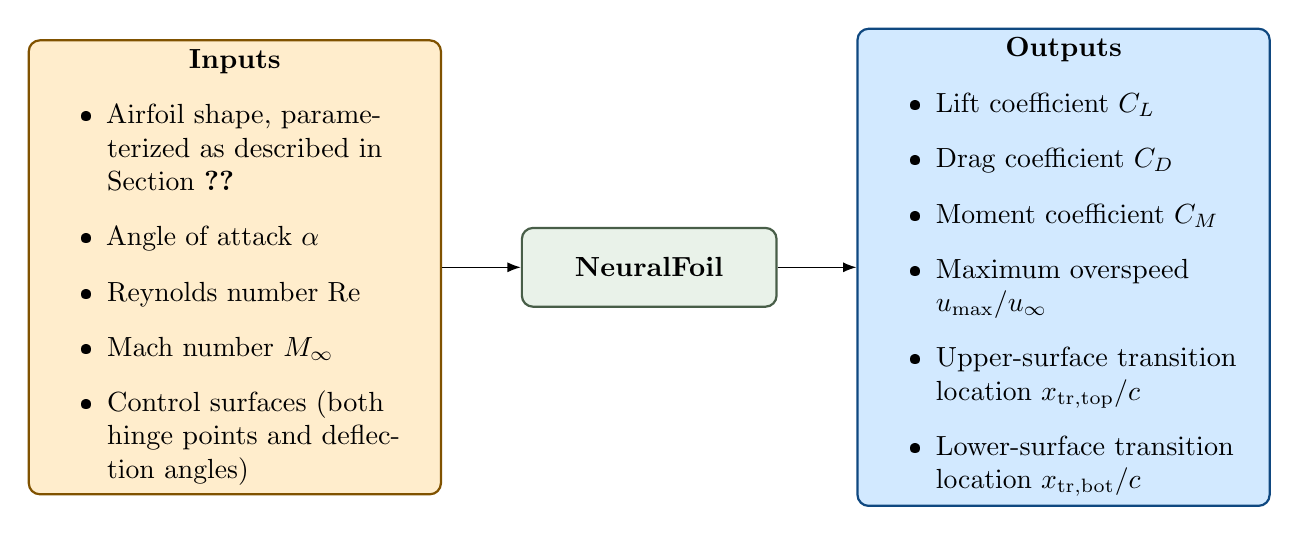
\begin{tikzpicture}[
            node distance=1 cm and 1 cm,
            auto,
            box/.style={
                rectangle,
                rounded corners,
                draw=#1!50!black,
                fill=#1!20,
                thick,
                text width=5cm,
                align=center,
                minimum height=1cm
            },
            title/.style={font=\bfseries},
            list/.style={align=left}
        ]

            % Nodes
            \node[box=myorange] (inputs) {
                \textbf{Inputs}
                \begin{itemize}
                    \item Airfoil shape, parameterized as described in Section \ref{sec:airfoil-parameterization}
                    \item Angle of attack $\alpha$
                    \item Reynolds number $\Rey$
                    \item Mach number $\Mi$
                    \item Control surfaces (both hinge points and deflection angles)
                \end{itemize}
            };

            \node[box=mydarkseagreen, right=of inputs, text width=3cm] (neuralfoil) {
                \textbf{NeuralFoil}
            };

            \node[box=mydodgerblue, right=of neuralfoil] (outputs) {
                \textbf{Outputs}
                \begin{itemize}
                    \item Lift coefficient $C_L$
                    \item Drag coefficient $C_D$
                    \item Moment coefficient $C_M$
                    \item Maximum overspeed $u_{\rm max} / u_\infty$
                    \item Upper-surface transition location $x_{\rm tr,top}/c$
                    \item Lower-surface transition location $x_{\rm tr,bot}/c$
                \end{itemize}
            };

            % Arrows
            \draw[-Latex] (inputs) -- (neuralfoil);
            \draw[-Latex] (neuralfoil) -- (outputs);
        \end{tikzpicture}
        \caption{User-facing inputs and outputs of the NeuralFoil model.}
        \label{fig:neuralfoil_io}
    \end{figure}

    NeuralFoil has a mathematical form that is fully explicit\footnote{meaning no iterative solvers are used} and guaranteed to produce a unique solution with a bounded amount of computational effort for any input. Reasonable aerodynamics estimates can be expected:
    \begin{itemize}
        \item For any practical airfoil shape\footnote{only single-element airfoils are allowed}, including modifications for trailing-edge control deflections up to reasonable deflections (e.g., $\pm 25\degree$)
        \item Across the $360\degree$ angle of attack range, by leveraging analytical post-stall models regressed from high-$\alpha$ wind tunnel data by Truong \cite{truong_analytical_2020}
        \item At any practical Reynolds number ($10^2$ to $10^9$) with physically-correct extrapolation even beyond these ranges (e.g., Stokes flow limit)
        \item At subsonic and transonic Mach numbers, from zero to slightly above the drag-divergent Mach number
    \end{itemize}

    NeuralFoil is implemented as an open-source lightweight Python package with minimal dependencies (only NumPy \cite{harris_array_2020} for the actual aerodynamic modeling), allowing easy installation across a variety of platforms.

    \subsection{Airfoil Geometry Parameterization}
    \label{sec:airfoil-parameterization}

    A user can specify input airfoil in many different forms -- for example, as an array of $(x, y)$ coordinates, as a standard \texttt{*.dat} file, or as an Airfoil-class object within the AeroSandbox aircraft design optimization framework \cite{sharpe_aerosandbox_2021}.

    However, underneath this interface layer, the actual airfoil geometry given to NeuralFoil's neural networks is parameterized as an 8-parameter-per-side CST (Kulfan) parameterization, with Kulfan's added leading-edge-modification (LEM) and trailing-edge thickness parameter \cite{kulfan_universal_2008, kulfan_modification_2020}. This gives a total of 18 parameters (corresponding to linear modes) to describe a given airfoil shape, which are illustrated in Figure \ref{fig:neuralfoil_parameterization}. This parameterization was chosen as Masters \cite{masters_geometric_2017} shows that this is one of the most parameter-efficient representations of airfoil shape and flexible enough to represent essentially all practical airfoil shapes. Kulfan's parameterization is strongly related to an orthogonal polynomial decomposition using Bernstein polynomials, which allows for its geometric flexibility. Moreover, this formulation, is linear and relatively interpretable, and is already common in existing aerospace tools such as OpenVSP \cite{mcdonald_open_2022}. Conversion of user-specified airfoils to this format for NeuralFoil to use is automatically and efficiently handled as a least-squares fitting problem.

    \begin{figure}[h]
        \centering
        \adjustbox{trim=0cm 1.5cm 0cm 0cm}{
            \includesvg[width=0.8\textwidth]{../../media/kulfan_parameterization_illustration.svg}
        }
        \caption{Geometry input parameterization used by NeuralFoil. Parameterization is an 18-parameter CST (Kulfan) parameterization. Each colored line in the figure represents a mode shape associated with one of these parameters; modes are linearly combined to form the airfoil shape.}
        \label{fig:neuralfoil_parameterization}
    \end{figure}

    \subsection{Model Architecture}

    At a high level, the mathematical model within NeuralFoil consists the following main steps:

    \begin{enumerate}
        \item Conversion of user airfoil shape into the required parameterization (including any control surfaces, which are made part of the airfoil geometry as described in Section \ref{sec:control-surfaces})
        \item Temporary restriction to the incompressible flow case (i.e., input Mach is set aside for now; addressed later)
        \item Transformation of user-facing inputs into an appropriate input vector space for the neural network
        \item A neural network that maps from this vector space to another vector space
        \item Transformation of this neural network output space back into the user-facing outputs
        \item Compressibility correction, which is described in Section \ref{sec:compressibility}
    \end{enumerate}

    The intermediate vector spaces described above are carefully parameterized such that relevant functions are closer-to-linear (and hence vastly easier for a neural network to learn) in these spaces than in the original user input and output spaces. Effectively, this is feature engineering using domain-specific knowledge, which is known to substantially increase model accuracy and parameter efficiency.

    For example, the user-facing input space (shown in Figure \ref{fig:neuralfoil_io}) is transformed into the following space, which is effectively what is seen by the neural network:

    \begin{equation}
        x_{\rm in,net} = \begin{bmatrix}
                             4 \sin(\alpha)                                 \\
                             20 \sin^2(\alpha)    \\
                             (\ln(\Rey) - 12.5) / 2 \\
                             (\text{Kulfan surface mode strengths}) \cdot 5             \\
                             (\text{Kulfan leading-edge weight}) \cdot 5    \\
                             (\text{trailing-edge thickness}) \cdot 100     \\
        \end{bmatrix}
    \end{equation}

    \noindent These quantities are physically-supported by closed form aerodynamic models, such as thin-airfoil theory before application of the small-angle limit, post-stall models by Truong \cite{truong_analytical_2020}, power-law dependency on Reynolds number stemming from Blasius and Falkner-Skan relations \cite{drela_aerodynamics_2019}, etc. Moreover, linear scaling factors are applied to all parameters such that their range of inputs are roughly on the order of magnitude of 1. This improves the stability of the neural network training process, and it improves the performance of the weight-decay-based regularization strategy that is later used during training to improve generalizability (described in Section \ref{sec:training-process}).

    NeuralFoil offers eight different deep neural network models, which offer a tradeoff between accuracy and computational cost. This tradeoff is implemented as differences in the number and size of hidden layers. Table \ref{tab:model-sizes} lists the different models, along with their number of hidden layers and neurons per hidden layer.

    \begin{table}
        \centering
        \caption{Neural network models offered in NeuralFoil.}
        \label{tab:model-sizes}
        \begin{tabular}{lll}
            \toprule
            Model        & Hidden Layers & Neurons per Hidden Layer \\ \midrule
            ``xxsmall''  & 2             & 32                       \\
            ``xsmall''   & 3             & 32                       \\
            ``small''    & 3             & 48                       \\
            ``medium''   & 4             & 64                       \\
            ``large''    & 4             & 128                      \\
            ``xlarge''   & 4             & 256                      \\
            ``xxlarge''  & 5             & 256                      \\
            ``xxxlarge'' & 5             & 512                      \\
            \bottomrule
        \end{tabular}
    \end{table}

    Each layer is a fully-connected linear layer. The activation function applied between each layer is a hyperbolic tangent function, which is chosen because the resulting model is infinitely smooth ($C^\infty$-continuous) and hence guaranteed to be amenable to later gradient-based design optimization.

    \subsubsection{Handling of Control Surface Deflections}
    \label{sec:control-surfaces}

    <Work complete, section to be written.>

    \subsubsection{Embedding of Angle of Attack Symmetry}

    <Work complete, section to be written; uses methods from Zhang \cite{zhang_threedimensional_2022}>

    \subsubsection{Fusion of Post-Stall Models}

    <Work complete, section to be written; uses methods from Truong \cite{truong_analytical_2020}>

    \subsubsection{Handling of Compressibility Effects}
    \label{sec:compressibility}

    At a high level, compressibility is handled by applying a correction factor to the incompressible results. This correction factor is computed using Laitone's rule \cite{laitone_new_1951}, which is a higher-order variant of the well-known Prandtl-Glauert and Karman-Tsien compressibility corrections. All of these compressibility corrections take two inputs: the pressure coefficient in the equivalent incompressible flow $\Cpo$ and the Mach number $M$; they return the pressure coefficient in the actual compressible flow $\Cp$. For comparison, all three corrections are given here, which conveniently show the higher-order terms retained in each successive relation:

    \begin{align}
        \label{eq:prandtl-glauert} \text{Prandtl-Glauert:} \qquad & \Cp = \frac{\Cpo}{\beta} \\
        \label{eq:karman-tsien} \text{Karman-Tsien:}\qquad    & \Cp = \frac{\Cpo}{\beta + \Mi^2 / (1 + \beta) \cdot \Cpo / 2} \\
        \label{eq:laitone} \text{Laitone \cite{laitone_new_1951}:}\qquad & \Cp = \frac{\Cpo}{\beta + \Mi^2 / \beta \cdot \Cpo / 2 \cdot \left( 1 + \frac{\gamma - 1}{2} \Mi^2 \right)}
    \end{align}

    \noindent where $\beta = \sqrt{1- \Mi^2}$, and $\gamma$ is the ratio of specific heats (1.4 for air near standard conditions). In theory, these compressibility corrections should apply only to the pressure-derived forces on the airfoil, while the shear forces are relatively unaffected. In practice, NeuralFoil does not have access to the breakdown ofpressure and shear forces, so this is not possible. Instead, NeuralFoil applies the compressibility correction to the lift force and pitching moment (which are pressure-dominated) but does not apply the correction to the drag force (which is often shear-dominated). This assumption, while relatively simple, proves to match compressible airfoil drag data computed with other methods quite closely, as shown in Section \ref{sec:validation_transonic}.

    Another useful definition is that of the sonic pressure coefficient $\Cpcr$, which is the pressure coefficient below which flow goes supersonic. This is derived from the isentropic relations, yielding:

    \begin{equation}
        \Cpcr = \frac{2}{\gamma \Mi^{2}} \left(
        \left(
        \frac{1 + \frac{\gamma - 1}{2} \Mi^{2}}{1 + \frac{\gamma - 1}{2}}
        \right)^{\frac{\gamma}{\gamma - 1}}
        - 1
        \right)
        \label{eq:sonic-pressure-coefficient}
    \end{equation}

    At the location where supersonic flow first begins at $\Mcr$, Equations \ref{eq:laitone} and \ref{eq:sonic-pressure-coefficient} can be set equal. This yields a relation that maps the minimum value of the incompressible pressure coefficient $\Cpm$ to the critical Mach number $\Mcr$. This relation does not admit a closed-form solution, but it can be solved numerically; results are shown in Figure \ref{fig:compressibility_corrections} for all three corrections.

    \begin{figure}[h]
        \centering
        \includesvg{./figures/critical_mach_vs_cp0.svg}
        \caption{Laitone's rule allows a mapping from the minimum incompressible pressure coefficient $\Cpom$ to the critical Mach number $\Mcr$.}
        \label{fig:compressibility_corrections}
    \end{figure}

    This implicit mapping is less desirable because the nonlinear solve is not guaranteed to converge, depending on initial guess. Instead, this relation can be replaced with an explicit surrogate model, which was obtained using symbolic regression (via PySR \cite{cranmer_interpretable_2023}):

    \begin{equation}
        \Mcr = \left(
        1.0083619
        - \Cpom
        + \left(-0.51058894 \cdot \Cpom \right)^{0.6553655}
        \right)^{-0.5536965}
        \label{eq:laitone_surrogate}
    \end{equation}

    Replacing the implicit mapping of Figure \ref{fig:compressibility_corrections} with the surrogate model of Equation \ref{eq:laitone_surrogate} introduces negligible error, with a corresponding RMS error in $\Mcr$ of $0.0014$ over all $\Cpom$ values. This relation allows NeuralFoil to estimate the critical Mach number $\Mcr$ using only incompressible quantities with surprising accuracy, often to within $\pm 0.01$ of results computed using the full-potential code MSES \cite{mses}. To determine $\Cpom$, which is needed for Equation \ref{eq:laitone_surrogate}, the definition of $\Cpom$ is used:

    \begin{equation}
        \Cpom = 1 - \left( \frac{u_{\rm max}}{u_\infty} \right)^2
    \end{equation}

    Following a derivation from Mason \cite{mason_transonic_2006}, an empirical relation for the shape of the drag rise beyond $\Mcr$ is included. Drag in this regime, especially beyond the drag-divergent Mach number $M_{\rm dd}$ is relatively simple and errs on the side of over-estimating wave drag. However, given that a primary goal of the NeuralFoil tool is to drive design optimization, this empirical model serves its purpose of steering the optimizer away from thick transonic airfoils with strong shocks.

    \subsection{Training Data Generation}
    \label{sec:training-data}

    Synthetic training data was generated by running XFoil on a large number of airfoils, spanning a wide range of angles of attack and Reynolds numbers. All training data is analyzed without compressibility in XFoil (i.e., $\Mi=0$); compressible effects were handled outside of the neural network training process, as described in Section \ref{sec:compressibility}.

    A stochastic procedure was used to generate the airfoil shapes used in training, and is described here:

    \begin{enumerate}
        \item First, three airfoils are randomly selected from the UIUC airfoil database \cite{uiuc_airfoil_database}. Three random weights are drawn, and the airfoils are linearly interpolated\footnote{precisely, the airfoils are converted to the Kulfan representation of Section \ref{sec:airfoil-parameterization} and these parameters are merged} based on these weights. As the UIUC database consists of roughly 1,650 airfoils, this procedure effectively ensures that each training airfoil is derived from a unique combination of three airfoils.
        \item This blended airfoil has its thickness uniformly scaled by a relative factor randomly drawn from $\operatorname{Lognormal}(\mu, \sigma^2)$, where $\mu=0$ and $\sigma=0.15$.
        \item Each of the Kulfan parameters described in Section \ref{sec:airfoil-parameterization} is perturbed by a random variable drawn from the product of a normal and exponential distribution; typical perturbations of these parameters are on the order of $\pm 0.05$.
        \item With 50\% probability, the airfoil is made to have a sharp trailing edge; otherwise, any nonzero trailing edge thickness is kept and perturbed by a small random amount on the order of $\pm 0.003$.
        \item With 75\% probability, the airfoil is made to have continuous leading-edge curvature (i.e., removing any sharp leading edge).
    \end{enumerate}

    In total, 12 million airfoil shapes were generated using this procedure. Airfoils were then analyzed using XFoil across a randomly-generated range of angles of attack and Reynolds numbers, both of which used a variety of statistical distributions to focus the training data on regions of interest but also include a substantial number of outliers. For example, the angles of attack included in the training data range from $-16.3\degree$ to $+17.1\degree$, and the Reynolds numbers range as low as 10 and and as high as 8.8 billion. Airfoil shape variation is sufficiently diverse that the XFoil-assessed lift coefficients range from $-1.86$ to $+3.28$.

    \subsection{Training Process}
    \label{sec:training-process}

    The neural networks at the heart of this approach were trained on a GPU computing cluster operated by the Lincoln Laboratory Supercomputing Center via MIT Supercloud. The training process was implemented using the PyTorch \cite{paszke_pytorch_2019} framework. The RAdam optimizer \cite{liu_variance_2019} was used with a decaying learning rate scheduled based on plateau of the training loss.

    Synthetic data generated using the procedure described in Section \ref{sec:training-data} was split into a training dataset (95\%) and a test dataset (5\%). The training dataset was used to train the neural network models, and the test dataset was used to evaluate the performance of the trained models and monitor for over-fitting. Critically, a small amount of weight decay (effectively, a $L^2$-norm penalty on all weight and bias parameters) was added to the loss function, which causes the network training to asymptote without over-fitting. Other alternatives that improve generalization, such as batch normalization and dropout, were tested; however, it was found that weight decay alone produced the models with the most accurate generalization to the test dataset.

    The loss function used when training the network is an $L^2$-norm composite of individual errors that each map to one of the user-facing outputs of Figure \ref{fig:neuralfoil_io}. The errors with respect to lift and drag are weighted most heavily in this loss function, as these are often the most important quantities for overall aircraft performance prediction.

    % TODO asymmetric CD penalty

    \subsection{Model Performance}

    \subsubsection{Sample Validation of NeuralFoil Accuracy vs. XFoil}
    \label{sec:validation_basic}

    Qualitatively, NeuralFoil tracks XFoil very closely across a wide range of angles of attack and Reynolds numbers. In Figure \ref{fig:clcd_polar}, we compare the performance of NeuralFoil to XFoil on aerodynamic polar prediction. In this test, both analyses are incompressible ($\Mi=0$); accuracy with compressible effects is addressed in the subsequent results (Section \ref{sec:validation_transonic}). Notably, the airfoil analyzed here was developed from scratch using an inverse design process for a real-world aircraft development program (\emph{Dawn One}, a high-altitude long-endurance aircraft \cite{sharpe_optimization_2021, sharpe_tailerons_2023}). In this sense, this airfoil is truly an out-of-distribution sample, as it is generated with an entirely separate process from the one used for training data. Because of this, NeuralFoil isn't gaining an unfair advantage by memorizing this airfoil's performance, so the results of Figure \ref{fig:clcd_polar} are representative of those achieved in practical design tasks. In this example, and in others, NeuralFoil's aerodynamic results are typically accurate to within a few percent of XFoil's predictions. NeuralFoil also has the benefit of smoothing out XFoil's ``jagged'' predictions (for example, near $C_L=1.4$ and $\Rey=90 \times 10^3$ in Figure \ref{fig:clcd_polar}) in cases where XFoil is not reliably converging, which would otherwise make gradient-based optimization essentially impossible.

    \begin{figure}[h]
        \centering
        \includesvg[width=\textwidth]{../../benchmarking/neuralfoil_point_validation.svg}
        \caption{Sample validation of NeuralFoil versus XFoil on an out-of-distribution airfoil.}
        \label{fig:clcd_polar}
    \end{figure}

    Table \ref{tab:neuralfoil_performance} quantifies the performance of NeuralFoil models with respect to XFoil more precisely. At a basic level, the figures of merit are accuracy (here, treating XFoil as a ``ground truth'') and computational speed. This table details both of these considerations.

    The first few columns show the error with respect to XFoil on the test dataset. As implied by the name, the test dataset is completely isolated from the training dataset, and NeuralFoil was not allowed to learn from the test dataset. Thus, the performance on the test dataset gives a good idea of NeuralFoil's accuracy on airfoil design tasks ``in the wild''.

    The second set of columns gives the runtime speed of the models, both for a single analysis and for a large batch analysis. Here, the benefit of NeuralFoil's vectorization is shown: for large batch analyses, runtimes many orders of magnitude faster than XFoil are possible, with minimal loss in accuracy.

    \begin{table}[h]
        \centering
        \caption{Performance comparison of NeuralFoil (``NF'') physics-informed machine learning models versus XFoil in terms of accuracy (treating XFoil as a ground truth) and speed. Runtime speeds are measured on an AMD Ryzen 7 5800H laptop CPU.}
        \label{tab:neuralfoil_performance}

        \begin{adjustbox}{width=\textwidth}

            \begin{tblr}{
                width=\textwidth,
                colspec={m{3cm} | m{2cm} m{2cm} m{2cm} m{2cm} m{2cm} m{2cm} | m{2cm} m{2cm}},
                row{1}={font=\bfseries},
%            column{1}={font=\bfseries},
            }
                \toprule
                Aerodynamics Model & \multicolumn{6}{m{12cm}}{Mean Absolute Error (MAE) of Given Metric, on the Test Dataset, with respect to XFoil} & \multicolumn{2}{m{4cm}}{Computational Cost to Run} \\ %\cmidrule{2-9}
                {}                     & Lift Coeff. & Fractional Drag Coeff. & Moment Coeff. & Max Overspeed                    & Top Transition Location & Bottom Transition Location & Runtime & Total Runtime \\
                {}                     & $C_L$       & $\ln(C_D)^{\dagger}$   & $C_M$         & $u_{\max}/u_{\infty}^{\ddagger}$ & $x_{tr, top}/c$   & $x_{tr, bot}/c$ & (1 run) & (100,000 runs) \\ \midrule
%                NF Linear $C_L$ Model & 0.116       & -                      & -             & -                                & -                   & -                  & 1 ms    & 0.020 sec      \\
                NF ``xxsmall''         & 0.065       & 0.121                  & 0.010         & 0.215                            & 0.073                   & 0.100                      & 3 ms    & 0.190 sec      \\
                NF ``xsmall''          & 0.042       & 0.075                  & 0.007         & 0.134                            & 0.039                   & 0.055                      & 4 ms    & 0.284 sec      \\
                NF ``small''           & 0.039       & 0.069                  & 0.006         & 0.122                            & 0.036                   & 0.050                      & 4 ms    & 0.402 sec      \\
                NF ``medium''          & 0.027       & 0.051                  & 0.004         & 0.088                            & 0.022                   & 0.033                      & 5 ms    & 0.784 sec      \\
                NF ``large''           & 0.024       & 0.045                  & 0.004         & 0.079                            & 0.020                   & 0.029                      & 6 ms    & 1.754 sec      \\
                NF ``xlarge''          & 0.023       & 0.043                  & 0.004         & 0.076                            & 0.019                   & 0.028                      & 10 ms   & 3.330 sec      \\
                NF ``xxlarge''         & 0.021       & 0.040                  & 0.003         & 0.071                            & 0.018                   & 0.025                      & 13 ms   & 4.297 sec      \\
                NF ``xxxlarge''        & 0.020       & 0.039                  & 0.003         & 0.070                            & 0.016                   & 0.024                      & 38 ms   & 8.980 sec      \\
                XFoil                  & 0           & 0                      & 0             & 0                                & 0                       & 0                          & 73 ms   & 42 min         \\ \bottomrule
            \end{tblr}
        \end{adjustbox}

        \begin{adjustbox}{width=\textwidth}
            \vspace{1pt}
            \begin{tblr}{
                width=\textwidth,
                colspec={l},
            }
                $^{\dagger}$ The deviation of $\ln(C_D)$ can be thought of as ``the typical relative error in $C_D$''. \\
                $^{\ddagger}$ This ``maximum overspeed'' gives $\Cpm$, which can be used to estimate the critical Mach number $M_\text{crit}$.\\
            \end{tblr}
        \end{adjustbox}

    \end{table}

    \subsection{Sample Validation on Transonic Case}
    \label{sec:validation_transonic}

    <Work complete, section to be written.>


    \section{Airfoil Design Optimization with NeuralFoil}

    Although the accuracy of NeuralFoil with respect to XFoil has been demonstrated in Section \ref{sec:validation_basic}, this alone is not sufficient to demonstrate that NeuralFoil is useful for design optimization. A major reason for this is that engineering design optimization is an adversarial process, where the optimizer aims to exploit not only the physics, but also the model errors. Exploitation of the physics is desirable and ultimately the goal of engineering design optimization, but exploitation of model errors leads to designs that are ostensibly promising but lose their luster when analyzed with other computational tools or built in real life.

    To assess whether a model such as NeuralFoil is prone to model error exploitation, we can set up a test problem with a known correct answer, and see how close the optimized result matches this. In aerodynamic shape optimization (and aircraft design more broadly), there are relatively few problems that are rigorously specified, and even fewer where an indisputable correct answer is provided. However, one such case study that provides a useful design problem is Drela's 1998 \textit{Pros \& Cons of Airfoil Optimization} \cite{drela_pros_1998}, which discusses airfoil design for the \emph{MIT Daedalus} human-powered aircraft \cite{langford_feasibility_1986, langford_daedalus_1989, drela_humanpowered_1985}. Basic figures for this aircraft, along with its centerline airfoil, the DAE-11, are shown in Figure \ref{fig:daedalus_iso}.

    \begin{figure}[h]
        \centering
        \includesvg[width=\textwidth]{figures/daedalus-iso.svg}
        \caption{}
        \label{fig:daedalus_iso}
    \end{figure}

    The design of the DAE-11 airfoil is effectively defined by the following airfoil design optimization problem; this formulation is taken directly from Drela \cite{drela_pros_1998} with minor modifications\footnote{specifically, a constant-$\Rey_c \sqrt{C_L}$ polar is used instead of a constant-$\Rey_c$ polar, the $C_M$ constraint is clarified to apply to all $C_L$ points, and the $\theta_{\rm TE}$ constraint is matched to the DAE-11 airfoil}:

    \begin{itemize}
        \item \textbf{Objective}: Minimize $C_{D, \mathrm{mean}}$ at $\mathrm{Re}_c = 500\mathrm{k} \cdot \left(\frac{C_L}{1.25}\right)^{-0.5}$ and $\mathrm{M}_\infty = 0.03$
        \begin{itemize}
            \item Where $C_{D, \mathrm{mean}}$ is the weighted average of $C_D$ values at $C_L = [0.8, 1.0, 1.2, 1.4, 1.5, 1.6]$, with relative weights of $[5, 6, 7, 8, 9, 10]$ at each respective $C_L$
        \end{itemize}
        \item \textbf{Variables}: airfoil shape and angle of attack $\alpha$
        \item \textbf{Constraints}:
        \begin{itemize}
            \item $C_M \geq -0.133$ (at all $C_L$ operating points)
            \item Trailing-edge angle $\theta_{\rm TE} \geq 6.03^\circ$ (allows manufacturability)
            \item Leading-edge angle $\theta_{\rm LE} = 180^\circ$ (prevents the formation of a sharp leading edge)
            \item At $x/c = 0.33$, $t/c \geq 0.128$ (to accommodate the main spar)
            \item At $x/c = 0.90$, $t/c \geq 0.014$ (to accommodate the rear spar)
        \end{itemize}
    \end{itemize}

    When posing airfoil design optimization problems (using NeuralFoil or with any other tool), it is often helpful to add basic regularization constraints; these tend to make airfoil optimization better-behaved by ruling out non-physical and unrealistic airfoils. For the simple airfoil design problem described above, these regularizations are not necessary and the optimizer will converge regardless. However, they are discussed here as ``best practices'' for airfoil optimization on more complicated problems:

    The first such constraint is that the airfoil thickness must be positive everywhere. This prevents the creation of self-intersecting airfoils, which can be analyzed in both XFoil and NeuralFoil, but are clearly not physically-valid shapes.

    The second such constraint aims to guide the optimizer away from airfoils that have excessively high local curvature, as these have boundary layer behavior that is quite difficult to predict. A useful quantitative metric for this behavior, termed the wiggliness $w$, is based on a metric by Wahba that has long proven successful in univariate spline regularization \cite{wahba_spline_2007}:

    $$w(\mathrm{airfoil}) = \int_0^1 \left( \frac{d^2}{dx^2} y_\mathrm{lower}(x) \right)^2 + \left( \frac{d^2}{dx^2} y_\mathrm{upper}(x) \right)^2 dx$$

    \noindent We can loosely approximate the spirit of this wiggliness measure from the discrete Kulfan parameterization as:

    $$w(\mathrm{airfoil}) \approx \sum_{i=2}^{N-1} \left(c_{\mathrm{lower},i+1} - 2 \cdot c_{\mathrm{lower},i} + c_{\mathrm{lower},i-1} \right)^2 + \left(c_{\mathrm{upper},i+1} - 2 \cdot c_{\mathrm{upper},i} + c_{\mathrm{upper},i-1} \right)^2$$

    \noindent where $c_{\mathrm{lower},i}$ and $c_{\mathrm{upper},i}$ are the $i$th Kulfan (CST) coefficients of the lower and upper surfaces, respectively. A reasonable heuristic for this regularization constraint is to restrict this metric to no more than four times that of the original initial guess airfoil (which is typically some generic airfoil, such as a NACA0010).

    Using the problem formulation described above, we can solve this airfoil design optimization problem by coupling NeuralFoil with the AeroSandbox aircraft design optimization framework \cite{sharpe_aerosandbox_2021}. This adds automatic differentiation capabilities to NeuralFoil, allowing efficient optimization using gradient-based methods. This optimization problem is solved in approximately 7 seconds on a standard laptop; the speed of this solution provides rapid feedback to the designer on how to improve the optimization problem formulation to capture design intent.

    Figure \ref{fig:daedalus_optimized} compares three airfoil designs, each aimed at solving the \emph{MIT Daedalus} airfoil design problem described previously:

    \begin{itemize}
        \item \textbf{NeuralFoil-optimized}, which is the result of optimizing while using NeuralFoil as the aerodynamics analysis tool
        \item \textbf{XFoil-optimized}, which is the result of optimizing while using XFoil as the aerodynamics analysis tool
        \item \textbf{Expert-designed}, which is the original DAE-11 airfoil designed by Drela \cite{drela_lowreynoldsnumber_1988} and used on the actual \emph{MIT Daedalus} aircraft
    \end{itemize}

    For comparison, Figure \ref{fig:daedalus_optimized} also includes the initial guess airfoil that was provided to the optimization algorithms (a simple NACA0012).

    \begin{figure}[h]
        \centering
        \includesvg[width=\textwidth]{figures/neuralfoil_daedalus.svg}
        \caption{NeuralFoil-optimized airfoils yield performance that is competitive with expert-designed airfoils and have qualitatively-similar shapes. Adversarial optimization is not observed, as the NeuralFoil-optimized and XFoil-optimized airfoils yield similar performance when analyzed using XFoil.}
        \label{fig:daedalus_optimized}
    \end{figure}

    The airfoil produced using NeuralFoil optimization is quite similar in shape to the those produced using XFoil optimization and expert-designed airfoils, when given the same design objectives and constraints. Likewise, aerodynamic performance is quite similar across all three airfoils. Notably, the aerodynamic polars depicted in Figure \ref{fig:daedalus_optimized} were produced by post-optimality analysis using XFoil. Given the minimal discrepancy between the NeuralFoil-optimized and XFoil-optimized airfoils, this suggests that NeuralFoil is not prone to model error exploitation.

    Interestingly, the differences between the expert-designed and optimized airfoils in Figure \ref{fig:daedalus_optimized} are attributable to design goals that were not factored into the quantitative problem formulation. For example, the optimized airfoils both exhibit a small amount of lower-surface concavity in the vicinity of $x/c \approx 0.15$, while the expert-designed DAE-11 has a flatter lower surface. Drela discusses reasons for this discrepancy in \cite{drela_pros_1998}, noting that concavity causes the wing covering (in the case of \emph{MIT Daedalus}, a thin covering of Mylar) to lift off of the surface of the wing (creating a bubble). This undesirable effect is not captured in the quantitative problem formulation, providing a cautionary tale that an optimized airfoil is only as good as the problem formulation that led to it.

    Nevertheless, the strength of NeuralFoil-powered optimization is that it allows one to generate optimized airfoils that are remarkably similar to expert-designed airfoils in mere seconds. This optimization capability is more-than-adequate for conceptual aircraft design, and it provides an excellent starting point for expert-guided airfoil design refinement.


    \section{Reproducibility Statement}

    All source code used in this paper is publicly available at \url{https://github.com/peterdsharpe/neuralfoil}. NeuralFoil itself is best accessed through the open-source AeroSandbox aircraft design optimization framework \cite{sharpe_aerosandbox_2021}; this provides some of the advanced features (e.g., $360\degree$ angle of attack, transonic effects, and control surface deflections) described in this work that are not yet available in the standalone NeuralFoil package.


    \section{Conclusion}
    \label{sec:conclusion}

    This paper introduces NeuralFoil, a physics-informed machine learning tool for airfoil aerodynamics analysis trained on an extensive dataset of XFoil analyses. NeuralFoil offers improved computational efficiency and optimization-friendliness while maintaining accuracy comparable to XFoil. Its ability to handle a wide range of practical airfoil shapes, angles of attack, Reynolds numbers, and Mach numbers up to low transonic conditions makes it a versatile tool in aerodynamic analysis.

    The accuracy of NeuralFoil with respect to XFoil is demonstrated across test cases, with particular focus on airfoils that NeuralFoil was not trained on (i.e., out-of-distribution). Much of the accuracy achieved here is due to the embedding of domain-specific physics knowledge into the model architecture, which increases the parameter-efficiency and generalizability of the resulting model. Also presented in this work is an application of NeuralFoil to airfoil design optimization for the MIT Daedalus human-powered aircraft, where it quickly produces designs close in performance and shape to expert-crafted airfoils. This showcases NeuralFoil's potential for rapid, accurate airfoil design optimization and iterative design processes.

    As a Python-based, open-source package, NeuralFoil offers a practical and versatile solution for applications in both academia and industry. Its robust performance, coupled with computational efficiency, positions it as a valuable asset for airfoil analysis and design, especially beneficial in the early stages of aircraft development where quick and reliable aerodynamic assessments are essential.

    \section*{Acknowledgments}
    The authors acknowledge the MIT SuperCloud and Lincoln Laboratory Supercomputing Center for providing high-performance computing resources that have contributed to the research results reported within this work.

    \bibliography{main, C:/Users/peter/Documents/Zotero/library, C:/Users/peter/Documents/Zotero/library-zotero}

\end{document}
